% CHECK: Lernziele
% • Sie können mindestens zwei Bereiche nennen, in
% denen Analogschaltungen heute in integrierten
% Schaltungen zur Anwendung kommen.
% • Sie kennen die Hauptschritte der Herstellung von
% integrierten Schaltungen in CMOS-Technologie.
% • Sie können die wichtigsten aktiven und passiven
% Bauelemente nennen und beschreiben, die in einem
% CMOS-Prozess standardmässig zur Verfügung
% stehen.

\section{CMOS Technologie}

% CHECK: [Flurin] This can be removed if unneded 
% [Simi] @Flurin I agree and threrefore it is outcommented :)

% \subsection{Geschichte} 
% \begin{description}
%     \item[1926] Julius E. Lilienfeld: Erster Vorschlag zur Realisierung eines SperrschichtFET
    
%     \item[1934] Oskar Heil: Erster Vorschlag eines Feldeffektverstärkers (Vorläufer vom MOSFET)
%     \item[1947] W. H. Brattain, J. Bardeen (und William B.Shockley): Erfindung des ersten Bipolartransistors
%     \item[1958] Jack S. Kilby: Erste Gedanken zur Realisierung einer integrierten Schaltung
%     \item[1961] Robert W. Noyce: Erhält Patent für die integrierte Schaltung
%     \item[1947] W. Shockley, J. Bardeen und W. Brattain: Erster funktionierender Bipolartransistor \rightarrow Physik-Nobellpreis
%     \item[1958] Jack S. Kilby: Erstes IC mit 1 Transistor, \qty{17.76}{\square\milli\meter}, Realisiert RC-Oszillator
%     \item[2024] Intel: Arrow Lake, >123\,Mio.Tr./mm$^2$
%     \item[2024] Apple: M4max, >92\,Mio.Tr./mm$^2$
% \end{description}

% \paragraph{Moores Law}
% 1965 hat G.E. Moore in einem Paper prognostiziert, dass sich die Transistorzahl pro chip in nächsten 10 Jahren jährlich verdoppeln wird. 
% 1975 wurde die Prognose revidiert auf eine Verdoppelung alle zwei Jahre.


\subsection{Prozessüberblick -- Herstellung integrierter Schaltungen}
Die Herstellung integrierter Schaltungen zeichnet sich durch folgende Besonderheiten aus:
\begin{itemize}
    \item Komplexe Logistik aufgrund einer Vielzahl an Prozessschritten
    \item Hochgradige Standardisierung
    \item Teure Infrastruktur und teure Prozesse
\end{itemize}

\smallskip

Der Prozess läuft in groben Zügen wie folgt ab:
\begin{enumerate}
    \item Sand wird geschmolzen und gereinigt. Daraus wird ein Silizium-Einkristall gezogen.
    \item Der Einkristall wird in Wafer geschnitten / gesägt.
    \item Durch wiederholte Oberflächenbeschichtung, Fotolithografie, Ätzen und Dotierung wird der Wafer strukturiert. Dazwischen muss der Wafer jeweils gesäubert werden.
    \item Die einzelnen Chips auf dem Wafer werden vereinzelt.
    \item Zur Konfektion werden die Chips in Gehäuse verbaut.
    \item Um die ICs in Systemen einzusetzen, werden diese auf Leiterplatten verbaut.
\end{enumerate}

\medskip

% NOTE: [Simi] I used the image from the script instead of the one from the slides (V1 S14)
% The one from the slides was not expotable in high quality (pdf) and the other image contains the same information...

\begin{minipage}[t]{0.5\columnwidth}
    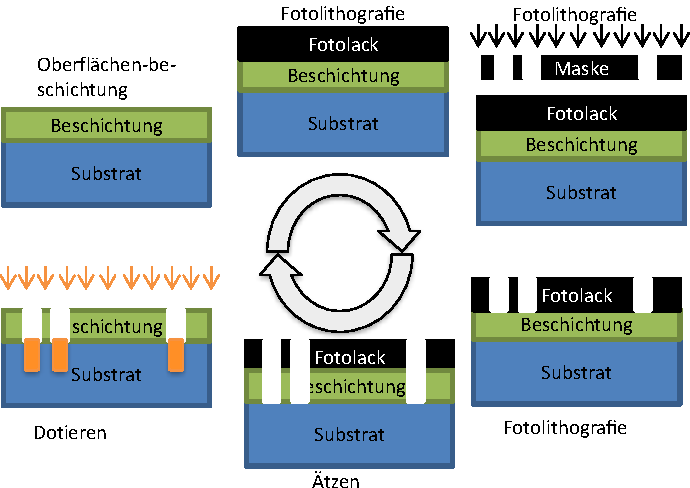
\includegraphics[width=\columnwidth, align=t]{images/technologie_grundprozess_skript.pdf}
\end{minipage}
\hfill
\begin{minipage}[t]{0.48\columnwidth}
    \paragraph{Lithographie}
    Lichtempfindlicher Lack (Photoresist) wird durch eine Lichtquelle löslich (positiver Photoresist) oder unlöslich (negativer Photoresist) gemacht.
    Durch Lösen des löslichen Photoresists kann die Oberfläche lokal geschützt werden und so gezielt regionen des Chips geätzt oder beschichtet werden.
    Zum Ende wird der übrige Lack entfernt und der Vorgang beliebig oft wiederholt.
\end{minipage}


% \paragraph{Lithographie}
% Das Prinzip der Lithographie basiert auf einem lichtempfindlichen Lack, dem sogenannten Photoresist.
% Dieser wird durch eine Lichtquelle löslich (positiver Photoresist) oder unlöslich (negativer Photoresist) gemacht.
% Durch lösen des löslichen Photoresists kann die Oberfläche lokal geschützt werden und so gezielt regionen des Chips geätzt oder beschichtet werden.
% Zum Ende wird der übrige Lack entfernt und der Vorgang beliebig oft wiederholt.


\paragraph{Ätzen}
Durch Ätzen kann gezielt Material von freiliegenden Flächen des Wafers entfernt werden.
Dabei werden folgende Verfahren unterschieden:
\begin{description}
    \item[Isotrop (Nass oder Plasma):] Gleichförmiges Ätzen in alle Richtungen \rightarrow Bringt die Gefahr des Unterätzens
    \item[Anisotrop (Reactive Ion Etching, KOH oder Plasma):] Ätzen entlang Kristallrichtungen, z.B. KOH greift die (111)-Ebene kaum an \rightarrow Ermöglicht steiliere Gräben, MEMS
    \item[Selektiv:] Selektives Ätzen bestimmter Materialien, z.B. HF ätzt SiO$_2$ aber nicht Si \\
        \rightarrow Erlaubt das Ätzen einer Lage ohne beschädigung unterliegender Strukturen
\end{description}

\paragraph{Dotieren}
Beim Dotieren werden gezielt Fremdatome in den Siliziumkristall eingebracht.
\begin{description}
    \item[Donatoren,] also Atome mit einem Valenzelektron mehr als der Halbleiter, verursachen einen Elektronenüberschuss, der Kristall wird \textbf{n-dotiert}.
    \item[Akzeptoren,] also Atome mit einem Valenzelektron weniger als der Halbleiter, verursachen einen Lochüberschuss, der Kristall wird \textbf{p-dotiert}.
\end{description}


\subsubsection{Backend Prozesse}

\paragraph{Wafer Sort}
Die Chips werden auf dem Wafer einzeln getestet (Kontaktierung mit Nadeln). 
Dies ist oft zeitaufwendig \rightarrow Durch gutes Design sollte diese Zeit minimiert werden.

Der Yield, (prozentualer Anteil funktionaler Chips) hängt dabei von der Chipgrösse ab.
Dies, da jeder Defekt bei grossen Chips eine grosse Fläche beeinträchtigt, da jeweils nur ganze Chips funktionsfähig oder defekt sein können.

Yields von \qty{90}{\percent} sind meist notwendig, um Profit zu machen.

\paragraph{Assembly and Test}
Die Wafer werden in einzelne Chips getrennt und die funktionierenden Chips in Gehäuse verbaut. Im Gehäuse erfolgt ein Final-Test.


\subsection{Arten von Toleranzen}
Bei der Herstellung von Wafern werden verschiedene Toleranzen unterschieden:
\begin{description}
    \item[Devicetoleranz] Toleranzen betreffend der Strukturen auf gleichem Chip
    \item[Prozesstoleranzen] Toleranzen betreffend der Strukturen auf einem Wafer
    \item[Lostoleranz] Toleranzen innerhalb eines Batches bzw. Los (meist 25, selten bis 50 Wafer)
\end{description}

\subsection{CMOS Bauelemente}
Mögliche Strukturen und Elemente wie auch die Materialeigenschaften werden im \textbf{Technologiehandbuch} gegeben.

%CHECK [Simi] @Flurin I have no idea how to compile the document with .svg files in it... therefore I added them as .pdf as well...?
% \subsubsection{NMOS und PMOS Transistoren}
% \begin{center}
%     \includesvg[scale=0.3]{images/01_CMOS.svg}
% \end{center}

% \subsubsection{Bipolartransistoren}
% \begin{center}
%     \includesvg[scale=0.3]{images/01_BJT.svg}
% \end{center}

\begin{minipage}[t]{0.48\columnwidth}
    \subsubsection{CMOS Transistoren}
    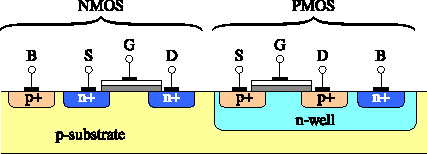
\includegraphics[width=\columnwidth, align=t]{images/01_CMOS.pdf}
\end{minipage}
\hfill
\begin{minipage}[t]{0.48\columnwidth}
    \subsubsection{Bipolartransistoren}
    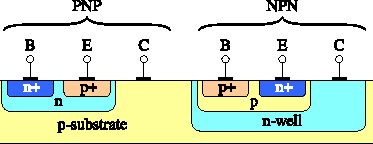
\includegraphics[width=\columnwidth, align=t]{images/01_BJT.pdf}
\end{minipage}


\subsubsection{Kapazitäten (pro Fläche)}

\vspace{-0.3cm}

$$ \boxed{ C = \varepsilon \cdot  \frac{A}{d} = \varepsilon_0 \cdot \varepsilon_r \cdot \frac{W \cdot L}{d} =  C'' \cdot A } \qquad \qquad
    \boxed{ C'' = \frac{\varepsilon}{d} = \frac{\varepsilon_0 \cdot \varepsilon_r}{d} } $$

\begin{minipage}[t]{0.44\columnwidth}
    \begin{tabular}{l@{}}
        $\varepsilon_0 = \qty{8.85e-12}{\farad\per\meter}$                      \\
        $\varepsilon_{r, \text{Si, SiO$_2$}} \approx 3.9$                       \\
        $\varepsilon_{r, \text{Dielektrikum}} \approx 2.9$ (möglichst klein)   
    \end{tabular}   
\end{minipage}
\hfill
\begin{minipage}[t]{0.55\columnwidth}
    \begin{tabular}{lll@{}}
        $C''$   & Spezifische Kapazität & $[C''] = \qty{}{\farad\per\square\meter}$ \\
        $A$     & Fläche der Kapazität  & $[A] = \qty{}{\square\meter}$             \\
        $d$     & Abstand (fix)         & $[d] = \qty{}{\meter}$
    \end{tabular}
\end{minipage}


% \[
%     \epsilon_0 = \qty{8.85e-12}{\farad\per\meter}
% \]
% \[
%     \epsilon_{r, \text{Si, SiO$_2$}} \approx 3.9
% \]
% \[
%     \epsilon_{r, \text{Dielektrikum}} \approx 2.9 \text{\ (Typisch, so klein wie möglich)}
% \]
% \[
%     C''\text{: Spezifische Kapazität}
% \]

\paragraph{MIM}
Metal-Interconnect-Metal-Kondensatoren produzieren \textbf{sehr kleine Kapazitäten}, da die Interconnect-Layers relativ dick sind ($d \sim \qty{2.5e-7}{\meter}$) und absichtlich aus 'schlechtem' Dielektrikum ($\varepsilon_r \approx 2.9$) bestehen.
Die Spannungsfestigkeit ist jedoch höher.

\paragraph{MOS}
Da Oxidschichten sehr dünn realisiert werden können ($d \sim \qty{2.33e-9}{\meter}$) und ein höheres $\varepsilon_r \approx 3.9$ besitzen, sind diese Kondensatoren bedeutend kleiner.
Sie besitzen jedoch eine kleinere Spannungsfestigkeit.
% CHECK: [Simi] @Flurin "sind diese Kondensatoren bedeutend kleiner" -> flächenmässig oder bezüglich ihrer Kapazität? 
% Ich hätte gesagt flächenmässig kleiner und können daher grössere Kapazitäten 'erzeugen'...? (V1 S23 / S24) 


\subsubsection{Spulen}
Spulen sind nur planar möglich und beanspruchen oft viel Platz.

\subsubsection{Widerstände (pro quadr. Flächeneinheit)}

\begin{minipage}[c]{0.48\columnwidth}
    $$ \boxed{ R = \rho \frac{L}{A} = \rho \frac{L}{t \cdot W} = R_\square \frac{L}{W} = R_\square \cdot n_\square } $$
    $$ \boxed{ R_\square = \frac{\rho}{t} } $$
\end{minipage}
\hfill
\begin{minipage}[c]{0.5\columnwidth}
    \paragraph{Typische Werte}

    \begin{tabular}{@{}l l@{}}
        Metall              & $R_\square \approx 0.02 ... \qty{0.08}{\ohm}$                  \\
        Poly (salicide)     & $R_\square \approx \qty{10}{\ohm}$                             \\
        Poly (non-salicide) & $R_\square \approx \qty{100}{\ohm}$ (n+ Poly)                  \\
                            & $R_\square \approx \qty{400}{\ohm}$ (p+ Poly)                  \\
        n- / p-Diffusion    & $R_\square \approx 100/\qty{150}{\ohm}$                        \\
        n- / p-Well         & $R_\square \approx 400/\qty{1600}{\ohm}$                       \\
    \end{tabular}
\end{minipage}


% \begin{center}
%     \boxed{
%         R = \rho \frac{L}{A} = \rho \frac{L}{t \cdot W} = R_\square \frac{L}{W}
%     }
% \end{center}
% \begin{center}
%     \boxed{
%         R_\square = \frac{\rho}{t}
%     }
% \end{center}


\subsubsection{Parasitäre Effekte}

\begin{minipage}[t]{0.7\columnwidth}
    \raggedright
    Widerstände und Kapazitäten weisen dieselben parasitären Effekte auf.

    \smallskip

    \textbf{Empfehlung: Verhältnisse verwenden, nicht Absolutwerte!}
\end{minipage}
\hfill
\begin{minipage}[t]{0.25\columnwidth}
    \begin{itemize}
        \item Streukapazitäten
        \item Toleranzen
        \item Nichtlinearitäten
    \end{itemize}
\end{minipage}


%TODO: Bilder zu den Parasitäten V1 S27
% [Simi] @Flurin: welche genau? Das mit dem Halbleiteraufbau UND das mit dem Schema?
